\chapter{Authenticated Encryption}

\todo{popis AEAD}

\section{Block cipher modes}

from 70s

\begin{description}
  \item[ECB]
  \item[CBC]
  \item[CFB]
  \item[OFB]
  \item[CTR]
\end{description}

\todo{Block cipher modes image from @angealbertini}

Exploiting malleability:

ECB: Rearrange, replay blocks
CTR, OFB: Bitwise modification of blocks
CBC: Change current ciphertext block to predictably change the next plaintext block (during decryption)

Chosen-boundary attacks:

ECB, CBC, CFB: Partial chosen-plaintext control
Decrypt messages byte by byte

Here come the XOR ninjas

\section{Authenticated Encryption}
\section{Authenticated Encryption with Associated Data}



\section{Generic compositions}

\begin{description}
  \item[Encrypt-and-MAC]
  \item[MAC-then-Encrypt]
  \item[Encrypt-then-MAC]
\end{description}

\begin{figure}
  \centering
  \begin{subfigure}[b]{0.3\textwidth}
    \centering
    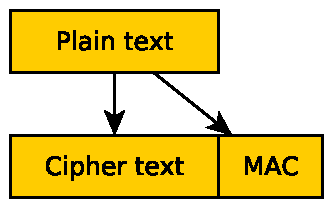
\includegraphics[width=0.9\textwidth]{images/encrypt-and-mac.pdf}
    \caption{Encrypt-and-MAC}
  \end{subfigure}
  \begin{subfigure}[b]{0.3\textwidth}
    \centering
    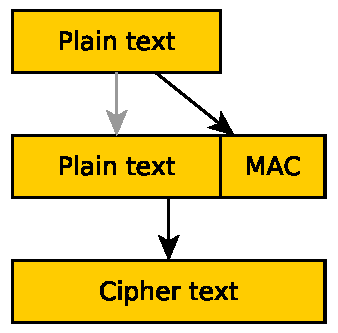
\includegraphics[width=0.9\textwidth]{images/mac-then-encrypt.pdf}
    \caption{MAC-then-encrypt}
  \end{subfigure}
  \begin{subfigure}[b]{0.3\textwidth}
    \centering
    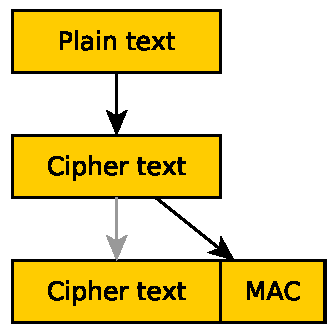
\includegraphics[width=0.9\textwidth]{images/encrypt-then-mac.pdf}
    \caption{Encrypt-then-MAC}
  \end{subfigure}
  \caption{Generic compositions of Authentized Encryption}
\end{figure}

\section{Competition for Authenticated Encryption: Security, Applicability and Robustness}

CAESAR is worldwide cryptographic competition, focused on finding new methods of authenticated encryption, that offer advantages against commonly used AES-GCM and will be suitable for widespread adoption. Submitted algorithms will be publicly evaluated by committee of researchers in fields of cryptography and cryptoanalysis.

\todo{popis algoritmů byly v soutěži, v čem se lišily, jaké a jak v nich byly nalezeny zranitelnosti a proto nepostoupily}

\todo{výběr algoritmu pro implementaci}

\subsection{Selection criteria}

\begin{description}
  \item[Online (one-pass)]
\end{description}



\subsection{NORX}

NO(T A)RX

ARX - Addition, Rotation, XOR

\subsubsection{Design goals}

\begin{itemize}
  \item \textbf{High security}
  \item \textbf{High speed} (in SW \textit{and} HW)
  \item \textbf{Simplicity} (of spec \textit{and} code)
  \item Online / one-pass
  \item Scalability (parallelism, unrolling)
  \item High key agility (no "key schedule")
  \item Side-channel leaks robustness (esp. timings)
\end{itemize}

\subsubsection{Parameters}

\begin{description}
  \item[Word Bit Size] $W \in {32, 64}$
  \item[Number of Rounds] $1 \leq R \leq 63$
  \item[Parallelism Degree] $0 \leq D \leq 255$ (0?)
  \item[Tag Bit Size] $|A| \leq 10W$
\end{description}

\begin{table}
  \centering
  \csvreader[
    after head=\begin{tabular}{llll}\toprule\csvlinetotablerow\\\midrule,
    late after line=\\,
    late after last line=\\\bottomrule\end{tabular}
  ]
    {tables/norx-proposed-instances.csv}{}
    {\texttt{\csvcoli} & \csvcolii & \csvcoliii & \csvcoliv}

  \caption{NORX proposed instances}
\end{table}

R=6: higher security margin

D=4: high throughput on parallel architectures

\subsection{Selection}

Benchmarks - Supercop, Brutus

\url{https://eprint.iacr.org/2014/850.pdf}
\url{http://www1.spms.ntu.edu.sg/~syllab/speed/}


